%%%%%%%%%%%%%%%%%%%%%%%%%%%%%%%%%%%%%%%%%
% Beamer Presentation
% LaTeX Template
% Version 1.0 (10/11/12)
%
% This template has been downloaded from:
% http://www.LaTeXTemplates.com
%
% License:
% CC BY-NC-SA 3.0 (http://creativecommons.org/licenses/by-nc-sa/3.0/)
%
%%%%%%%%%%%%%%%%%%%%%%%%%%%%%%%%%%%%%%%%%

%----------------------------------------------------------------------------------------
%	PACKAGES AND THEMES
%----------------------------------------------------------------------------------------

\documentclass[aspectratio=169,usenames,dvipsnames]{beamer}

\usepackage[utf8]{inputenc}
\usepackage{booktabs}
\usepackage{tabularx}
\usepackage[authordate,bibencoding=auto,strict,backend=biber,natbib]{biblatex-chicago}
\addbibresource{bib.bib}
\usepackage{graphicx}
% \hypersetup{
%     colorlinks,
%     %citecolor=black,
%     linkcolor=black
% }
\usepackage{array}
\usepackage{caption}
\usepackage{threeparttable}
\usepackage{epigraph} 
\usepackage{lscape}
\usepackage{adjustbox}
\newcommand*{\Scale}[2][4]{\scalebox{#1}{\ensuremath{#2}}}%
\usepackage{import}
\newenvironment{wideitemize}{\itemize\addtolength{\itemsep}{10pt}}{\enditemize}
\usepackage{amsmath}
\usepackage{csvsimple}
\usepackage{siunitx}
\usepackage{filecontents}
\usepackage{rotating}
\usepackage{multirow}
\usepackage{amsmath}
\usepackage{subcaption}
\usepackage{appendixnumberbeamer}
\usepackage{float}
\usepackage{amsmath}
\usepackage{csvsimple}
\usepackage{hyperref}
\newtheorem{proposition}{Proposition}
\usepackage{xcolor}
\def\boxit#1#2{%
    \smash{\color{red}\fboxrule=1pt\relax\fboxsep=2pt\relax%
    \llap{\rlap{\fbox{\phantom{\rule{#1}{#2}}}}~}}\ignorespaces
}
\newenvironment{variableblock}[3]{%
  \setbeamercolor{block body}{#2}
  \setbeamercolor{block title}{#3}
  \begin{block}{#1}}{\end{block}}
\usepackage{appendixnumberbeamer}
\usepackage{tikz,pgfplots}
\usepackage{tkz-fct}
\usepackage{amsthm}
\pgfplotsset{compat=1.10}
\usepgfplotslibrary{fillbetween}
\mode<presentation> {
\AtBeginSection[]
{
    \begin{frame}
        \frametitle{Table of Contents}
        \tableofcontents[currentsection]
    \end{frame}
}
% The Beamer class comes with a number of default slide themes
% which change the colors and layouts of slides. Below this is a list
% of all the themes, uncomment each in turn to see what they look like.

\usetheme{default}
%\usetheme{AnnArbor}
%\usetheme{Antibes} -
%\usetheme{Bergen}
%\usetheme{Berkeley}
%\usetheme{Berlin}
%\usetheme{Boadilla}
%\usetheme{CambridgeUS}
%\usetheme{Copenhagen} -
%\usetheme{Darmstadt}
%\usetheme{Dresden}
%\usetheme{Frankfurt}
%\usetheme{Goettingen}
%\usetheme{Hannover}
%\usetheme{Ilmenau}
%\usetheme{JuanLesPins}
%\usetheme{Luebeck}
%\usetheme{Madrid}
%\usetheme{Malmoe}
%\usetheme{Marburg}
%\usetheme{Montpellier}
%\usetheme{PaloAlto}
%\usetheme{Pittsburgh}
%\usetheme{Rochester} -
%\usetheme{Singapore}
%\usetheme{Szeged}
%\usetheme{Warsaw}

% As well as themes, the Beamer class has a number of color themes
% for any slide theme. Uncomment each of these in turn to see how it
% changes the colors of your current slide theme.

%\usecolortheme{albatross}
%\usecolortheme{beaver}
%\usecolortheme{beetle}
%\usecolortheme{crane}
%\usecolortheme{dolphin}
%\usecolortheme{dove}
%\usecolortheme{fly}
%\usecolortheme{lily}
%\usecolortheme{orchid}
%\usecolortheme{rose}
%\usecolortheme{seagull}
%\usecolortheme{seahorse}
%\usecolortheme{whale}
%\usecolortheme{wolverine}

%\setbeamertemplate{footline} % To remove the footer line in all slides uncomment this line
%\setbeamertemplate{footline}[frame number] % To replace the footer line in all slides with a simple slide count uncomment this line
\setbeamertemplate{theorems}[numbered]
\setbeamertemplate{navigation symbols}{} % To remove the navigation symbols from the bottom of all slides uncomment this line
}
\setbeamertemplate{caption}{\raggedright\insertcaption\par}
  \setbeamertemplate{enumerate items}[default]
  %\setbeamertemplate{page number in head/foot}{\insertframenumber}
\usepackage{graphicx} % Allows including images
\usepackage{booktabs} % Allows the use of \toprule, \midrule and \bottomrule in tables
%\usepackage {tikz}
\newtheorem*{theorem*}{Theorem}
\newtheorem*{lemma*}{Lemma}
\newtheorem*{proposition*}{Proposition}
\newtheorem*{corollary*}{Corollary}
\newtheorem*{definition*}{Definition}
\DeclareMathOperator*{\argmin}{arg\,min}
\newtheorem*{assumption}{Assumption}
\usetikzlibrary {positioning}
\renewcommand{\arraystretch}{1.5}
\newcommand\hideit[1]{%
  \only<0| handout:1>{\mbox{}}%
  \invisible<0| handout:1>{#1}}
\usepackage[default]{lato}

\setbeamercolor{block body alerted}{bg=alerted text.fg!10}
\setbeamercolor{block title alerted}{bg=alerted text.fg!20}
\setbeamercolor{block body}{bg=structure!10}
\setbeamercolor{block title}{bg=structure!20}
\setbeamercolor{block body example}{bg=green!10}
\setbeamercolor{block title example}{bg=green!20}


\makeatletter
\let\save@measuring@true\measuring@true
\def\measuring@true{%
  \save@measuring@true
  \def\beamer@sortzero##1{\beamer@ifnextcharospec{\beamer@sortzeroread{##1}}{}}%
  \def\beamer@sortzeroread##1<##2>{}%
  \def\beamer@finalnospec{}%
}
\makeatother
%\usepackage {xcolor}

%----------------------------------------------------------------------------------------
%	TITLE PAGE
%----------------------------------------------------------------------------------------

\title[diss]{Lecture 8: Gaming the System} % The short title appears at the bottom of every slide, the full title is only on the title page
\author{Compensation in Organizations} % Your name
\institute[shortinst]{Jacob Kohlhepp}
\date{\today} % Date, can be changed to a custom date

\begin{document}

\begin{frame}
\titlepage % Print the title page as the first slide

\end{frame}

\section{Gaming by Timing Sales}


\begin{frame}{Oyer (1998) ``Fiscal year Ends and Nonlinear Incentive Contracts"}

\begin{wideitemize}
    \item Many performance pay contracts observed in practice are nonlinear.
    \begin{wideitemize}
        \item Salespeople get a discrete bonus when they achieve quote, execs. start getting bonus when they hit a profitability threshold.
    \end{wideitemize}
    \item This creates an incentive to strategically delay or speed up sales.
    \item Crucially fiscal year ends vary across firms.
    \item Main result: across the economy, sales are lower in the beginning of a firm's fiscal year and higher at the end.
\end{wideitemize}
\end{frame}


\begin{frame}[c]{Oyer (1998): Example of Non-Linear Incentives }
\centering
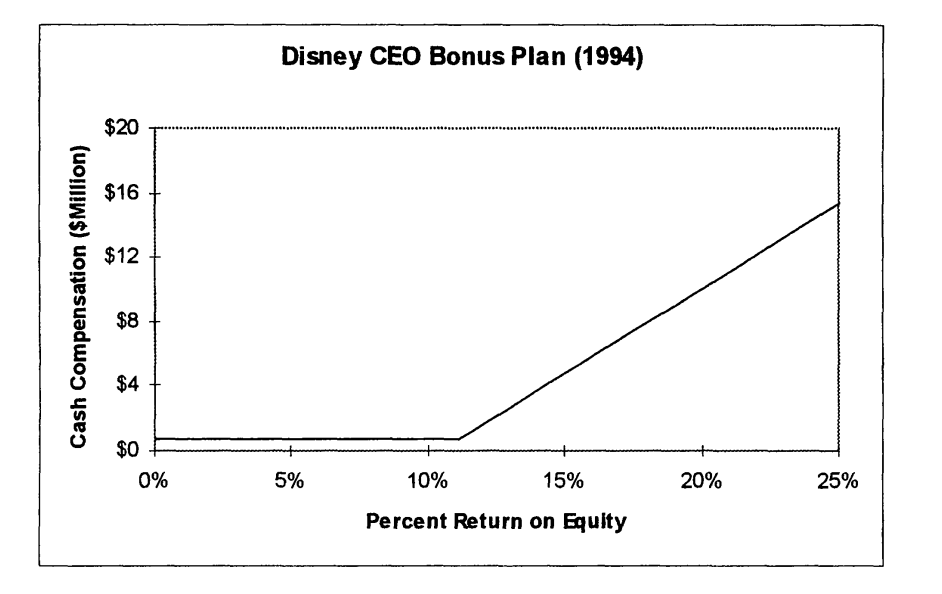
\includegraphics[width=0.9\textwidth]{pictures/oyer_example.png}

\end{frame}

\begin{frame}[c]{Oyer (1998): Example of Two Competing Firms}
\centering
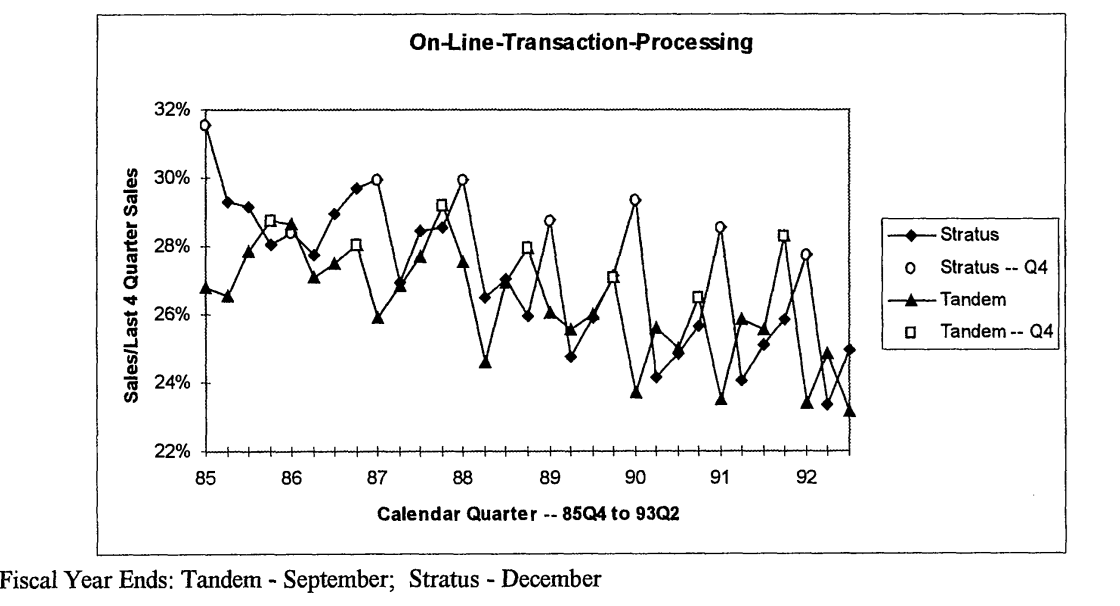
\includegraphics[width=0.9\textwidth]{pictures/oyer_suggestive.png}

\end{frame} 

\begin{frame}[c]{Oyer (1998): Impact of Fiscal Year End on Sales (All Manufacturing Firms) }
\centering
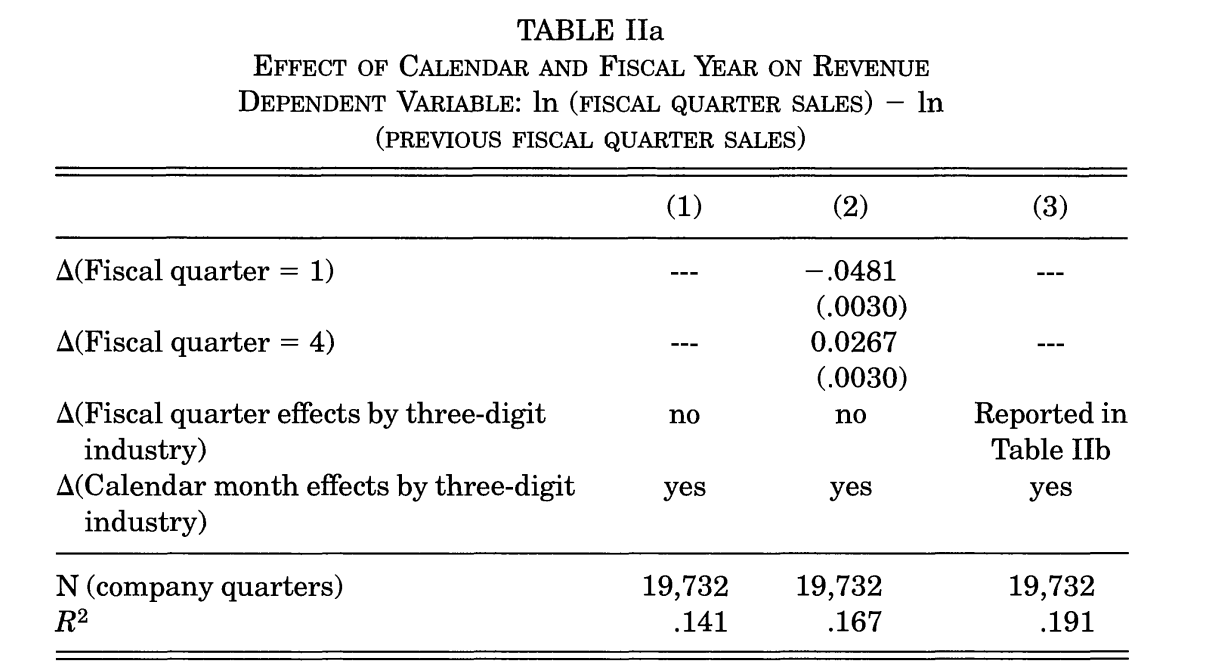
\includegraphics[width=0.9\textwidth]{pictures/oyer_main.png}

\end{frame}

\begin{frame}[c]{Oyer (1998): Impact of Fiscal Year End on Prices (All Manufacturing Firms) }
\centering
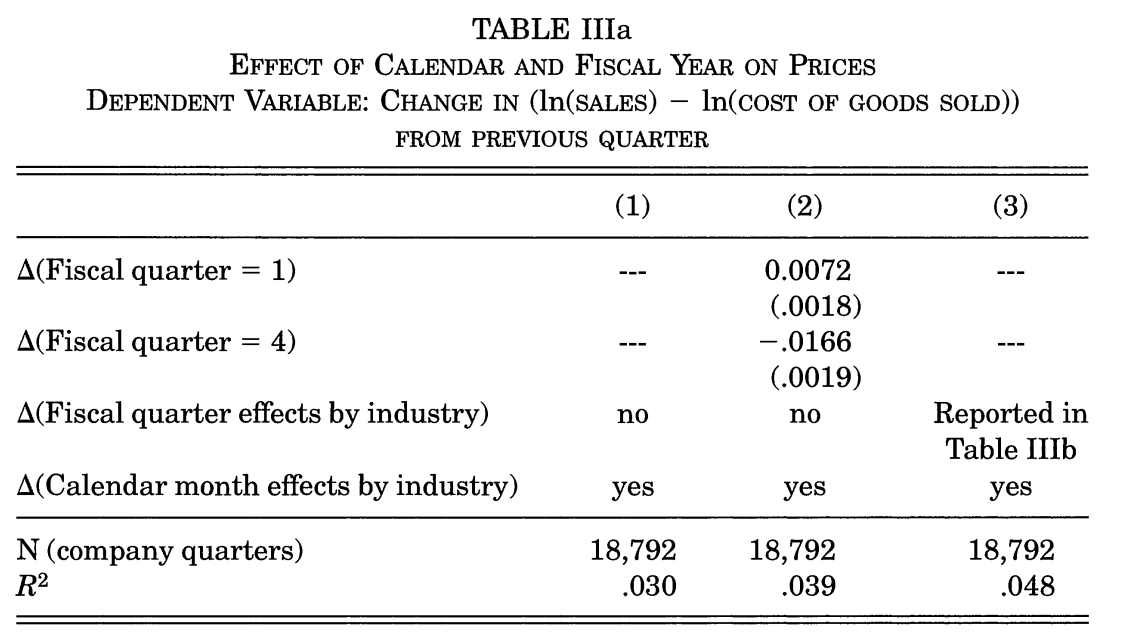
\includegraphics[width=0.9\textwidth]{pictures/oyer_price.png}

\end{frame}

\begin{frame}
\centering
    \huge Discussion: Larkin (2014)
\end{frame}


\begin{frame}{``The Cost of High-Powered Incentives" (Larkin 2014)}

\begin{wideitemize}
    \item Setting: enterprise software salespeople between 1997 and 2003
    \item Salespeople only close between 1-2 deals a quarter (often they close 0)
    \item But deals are massive: median deal is \$350,000
    \item Performance pay is nonlinear (so gaming is possible)
    \item Salespeople had the ability to discount prices.
    \item Nearly 67\% of deals closed the last day of the quarter
\end{wideitemize}
\end{frame}

\begin{frame}[c]{Larkin (2014): Nonlinear Pay (Accelerators)}
\centering
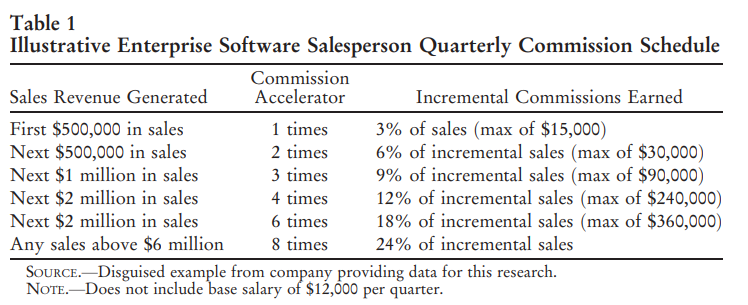
\includegraphics[width=0.7\textwidth]{pictures/larkin_accelerator.png}

\end{frame}


\begin{frame}[c]{Larkin (2014): Suggestive Evidence of Discounting}
\centering
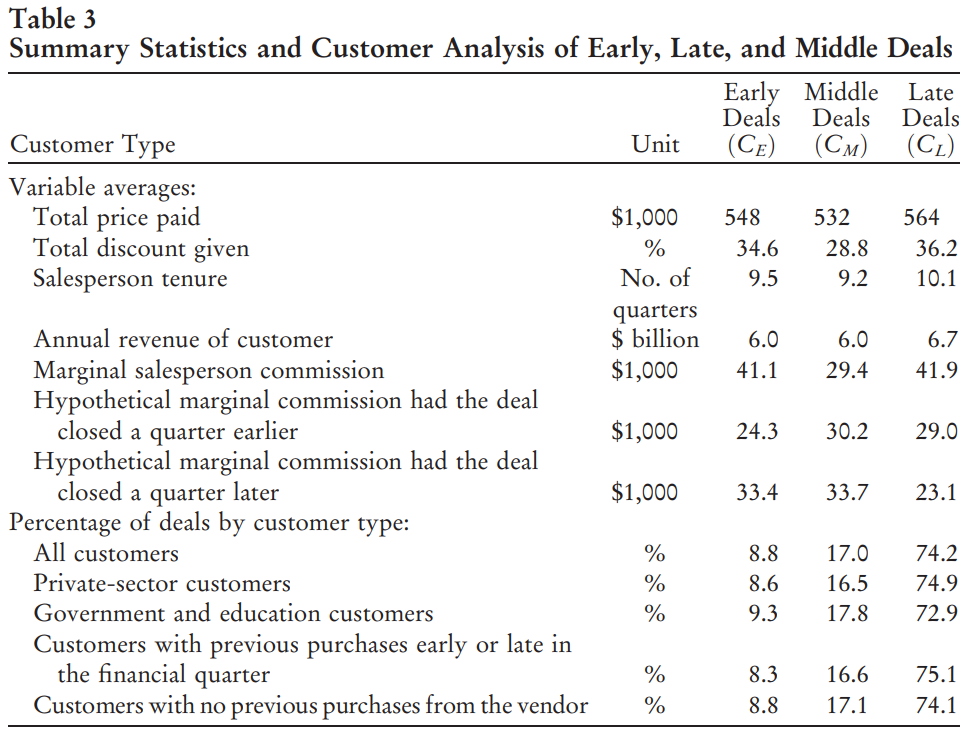
\includegraphics[width=0.7\textwidth]{pictures/larkin_suggestive.png}

\end{frame}

\begin{frame}[c]{Larkin (2014): Pushing and Pulling Deals}
\centering
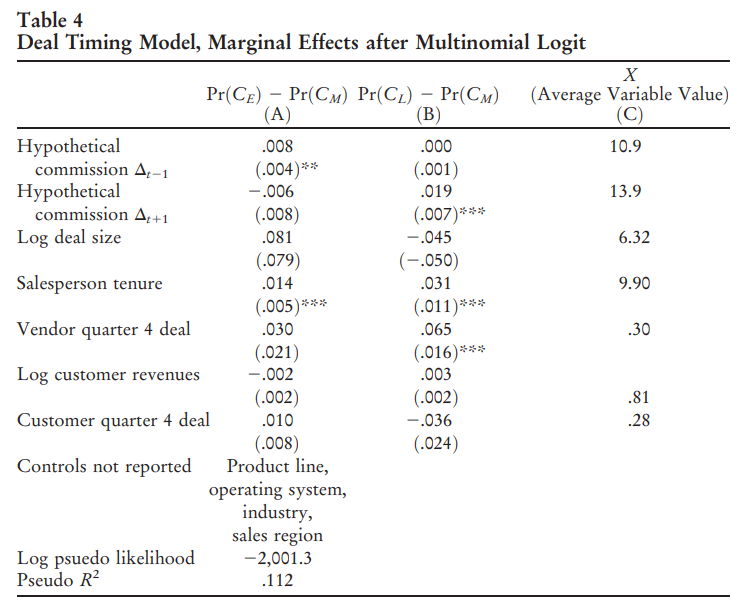
\includegraphics[width=0.7\textwidth]{pictures/larkin_pushpull.png}

\end{frame}

\begin{frame}[c]{Larkin (2014): Discounting Price to Close Faster}
\centering
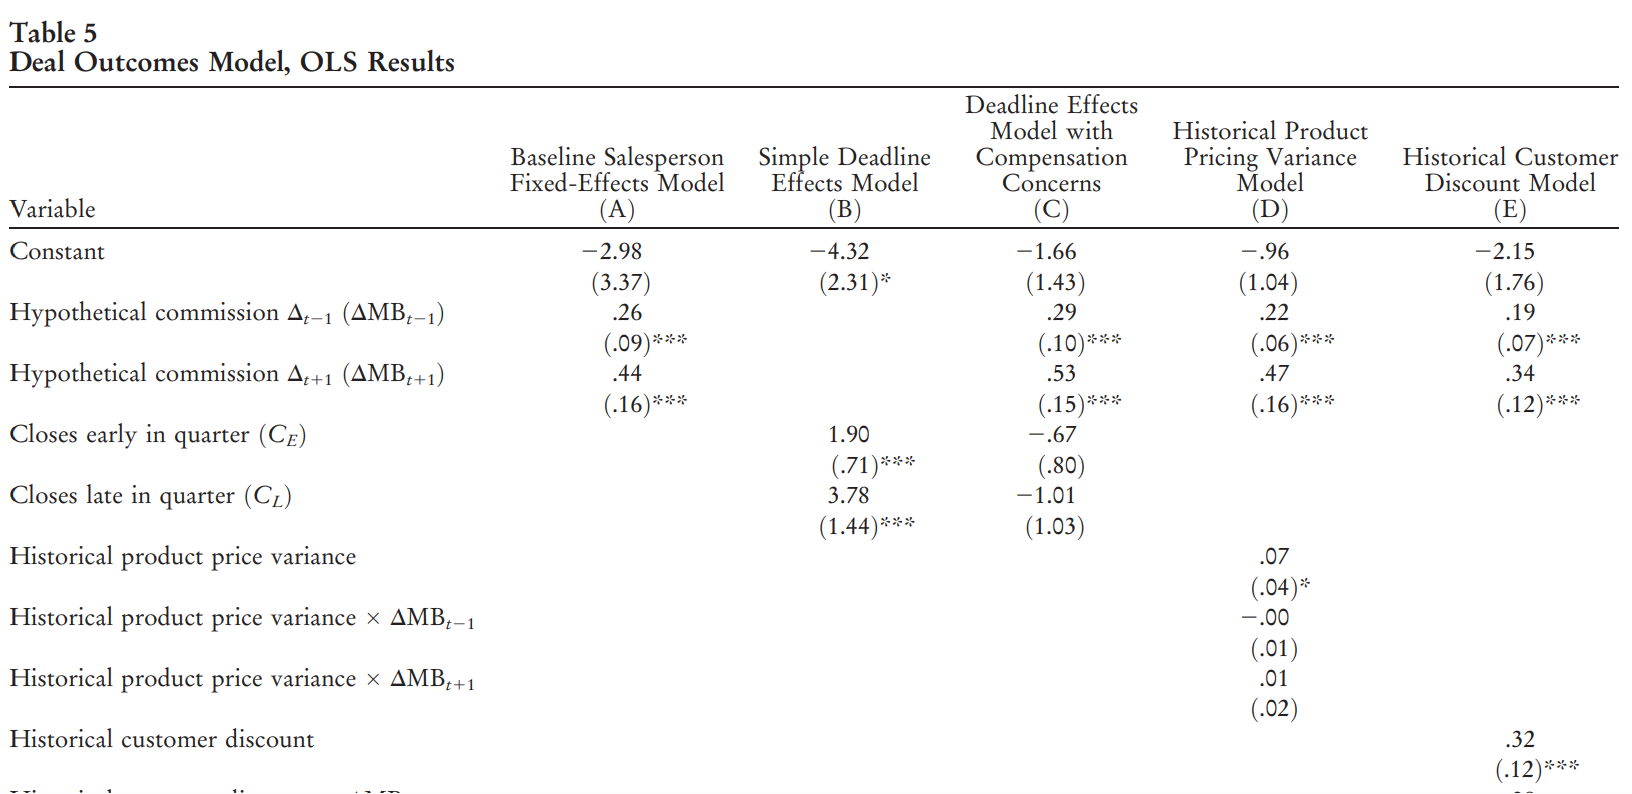
\includegraphics[width=0.9\textwidth]{pictures/larkin_discount.png}

\end{frame}


\begin{frame}{Larkin (2014): Summary}

\begin{wideitemize}
    \item Salespeople push or pull deals to manipulate the pay scheme.
    \item Estimated cost to revenue is between 5.69\% and 8.65\%
    \item Main challenge: is this gaming or price discrimination?
    \item The paper addresses this indirectly but cannot fully rule it out.
    \item Nonlinear incentive schemes cause these sorts of problems.
    \item This is one reason to use linear compensation!
\end{wideitemize}
\end{frame}

\section{The Ratchet Effect}

\begin{frame}{Roy (1952)}
\begin{wideitemize}
    \item Sociologist Donald Roy worked ``undercover" in a steel-processing plant for 11 months.
    \item He kept a journal of his production and observations.
    \item The plant used piece rates (performance pay).
    \item His earnings fluctuated from \$0.09 to \$1.66 per hour.
    \item Importantly, his hourly earnings were bimodal: he did two ``types" of work.
\end{wideitemize}
\end{frame}

\begin{frame}{Roy (1952)}
\begin{wideitemize}
    \item Half the time he produced well above his base rate.
    \item Half the time he produced well below.
    \item The distributions are almost completely separate.
    \item Other workers ancedotally reported doing this too.
    \item Some possible reasons:
    \begin{wideitemize}
        \item learning to do the job.
        \item Hard vs. easy work.
        \item others?
    \end{wideitemize}
\end{wideitemize}
\end{frame}

\begin{frame}[c]{Roy (1952): The Real Reason}
 Roy gives a different reason: workers intentionally slacked off to avoid a time study:
 \centering
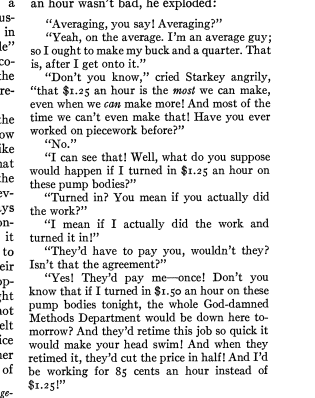
\includegraphics[width=0.4\textwidth]{pictures/roy_ratchet.png}
\end{frame}


\begin{frame}[c]{Roy (1952): The Real Reason}
This gave rise to even more blatant slacking off at night:
\centering
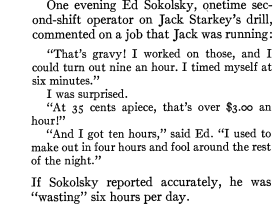
\includegraphics[width=0.4\textwidth]{pictures/roy_night.png}

\end{frame}




\begin{frame}{Return to Our Base Model}

\begin{wideitemize}
    \item Recall the performance pay model ($w(y)=\alpha+\beta y$)
    \item What exactly must the firm know to set compensation?
    \item Recall your homework exercise for the case when $E[\epsilon] = \bar y$, with cost that is $c(e)=e^2/2$:
    \[\alpha = \bar u+\frac{r\beta^2 \sigma^2}{2}-\beta (e+\bar y) -\frac{e^2}{2}\]
    \item The firm needs to know average output absent extra effort: $E[\epsilon]=\bar y$
\end{wideitemize}
    
\end{frame}


\begin{frame}{Measuring $\bar y$}

\begin{wideitemize}
    \item How can the firm measure $\bar y$?
    \item Set some arbitrary $\beta, \alpha$ which is NOT $\alpha_P, \beta_P$
    \item Then the firm knows that $e=\beta$ (why?)
    \item Then we have that:
    \[y = e + \epsilon \leftrightarrow E[y] = e + \bar y \leftrightarrow \bar y  = E[y]-e\]
    \item The firm can get $E[\epsilon]$ by subtracting effort from average output!
\end{wideitemize}
    
\end{frame}

\begin{frame}{Measuring $\bar y$}
\begin{wideitemize}
    \item How do we estimate this?
    \item For $i=1,...,N$ days, set the piece rate to be some $\beta$.
    \item Then measure output and compute the following:
    \[ \hat{ y}_N = \frac{1}{N}\sum_{i=1}^N  y_i -  \beta \]
    \item As we get enough data the law of large numbers means that:
    \[ \lim_{N\to \infty} \frac{1}{N}\sum_{i=1}^N  y_i = E[y] \implies \lim_{N\to \infty} \hat{ y}_N = \bar y \]
\end{wideitemize}
    
\end{frame}

\begin{frame}{The Ratchet Effect: Using Past Performance for Future Pay}
    \begin{wideitemize}
    \item After learning $\bar y$, the firm can set the ``right" $\alpha=\alpha_P$:
    \[\alpha_P = \bar u+\frac{r\beta_P^2 \sigma^2}{2}-\beta_P (e_P+\bar y) -\frac{e_P^2}{2}\]
    \item But what if employees know that the firm is doing this?\pause 
    \item They can choose reduce effort $e=\beta-\delta $ and then:
    \[ \lim_{N\to \infty} \hat{y}_N = \bar y - \delta\]
    \item The firm underestimates $\bar y$ and overpays workers:
\[\alpha_{actual} = \alpha_P+\beta_P \delta   \]
\end{wideitemize}

\end{frame}



\section{Does Gaming Matter?}

\begin{frame}{Does It Matter?}
    \begin{wideitemize}
        \item Gaming only matters if it lowers total surplus.
        \item For example: if sales people work harder the last part of a quarter and less hard during the beginning this is not necessarily destructive.
        \item But if they are working less hard overall this could be destructive.
        \item Or if time spent gaming the system takes time away from something productive.
        \item Question: What are examples of ``destructive" gaming?
        \item Question: What are examples of harmless gaming?
    \end{wideitemize}
\end{frame}

\begin{frame}{``An Empirical Investigation of Gaming Responses to Explicit Performance Incentives" (Courty and Marschke 2004)}

\begin{wideitemize}
    \item Question: Does gaming actually decrease welfare?
    \begin{wideitemize}
        \item ``The main goal of this article is to examine whether this behavior reflects a misallocation of real resources or simply an accounting phenomenon."
    \end{wideitemize}
    \item Contribution: Other papers show gaming happens but it is unclear if it hurts welfare.
    \item The Job Training Partnership Act (JTPA) gave performance pay to federal bureaucrats.
    \item Specifically, agencies get rewards for the labor market outcomes of the people they train.
    \item But, agencies can choose the timing of graduation (there is room for gaming)
\end{wideitemize}
\end{frame}

\begin{frame}{More About the JTPA (Courty and Marschke 2004)}

\begin{wideitemize}
    \item The largest federal employment and training program with \$4 billion budget and nearly a million people trained per year.

    \item Carried out by 620 smaller agencies with a lot of discretion.
    \item Performance measures (for agency): employment status, wage, earnings, number of weeks worked.
    \item Measured on date of graduation (which agencies can choose).
    \item Graduation date must be within 90 days of last training day.
    \item Most rewards are base don just meeting a minimum standard.
    \item Rewards were on average 7\% of participant budgets.
\end{wideitemize}
\end{frame}


\begin{frame}{Gaming the JTPA (Courty and Marschke 2004)}
\begin{wideitemize}
    \item Theoretically, the agencies want to game the system this way:
    \begin{wideitemize}
    \item Graduate everyone who is employed on the first day they are employed.
    \item Graduate people who are never employed on the last possible day (day 90).
\end{wideitemize}\pause
\item They game the system: on average employed people graduate 34 days earlier.
\item And the strategy they use is statistically similar to the optimal strategy.
\item Only big difference is that agencies wait 101.8 days on average for unemployed (so the 90 day window seems to not be enforced well).
\item Employment outcomes would be 20\% lower if they graduate people on the last day of training.
\end{wideitemize}

\end{frame}

\begin{frame}{Gaming Impacts Welfare (Courty and Marschke 2004)}
\begin{wideitemize}
    \item Agencies also graduate workers sooner or later (in the current fiscal year or next) in order to meet the standard this year or next.
    \item This more subtle manipulation seems to hurt worker welfare.
    \item Specifically delaying graduating leads to reduced length of training.
    \item The authors estimate 1 day delay in graduation on average reduces earnings gains by \$47 for the median enrollee.
\end{wideitemize}

\end{frame}

\end{document}







